\section{Experiment 4 and 5 - Adjusting Parameters}
\label{sec:phase3}
In this set of experiments the fitness functions $F_{basic}^{min}$ \eqref{eq:FBasicMin} and $F_{edge}^{min}$ \eqref{eq:FEdgeMin} are tested again on the small synthetic dataset 1 and the healthcare dataset, but with an adjusted setup as shown in table \ref{tab:setup3}. The setup is relaxing the objective for minimizing the role model complexity (role count, assignment counts).

\begin{table}[H]
    \centering
    \begin{tabular}{|l|l|}
        \hline
        \rowcolor{myGray} 
        \textbf{Parameter}              & \textbf{Value}    \\ \hline
        Generations                     & 1000              \\ \hline
        Population                      & 1000              \\ \hline
        CXPB                            & 0.25              \\ \hline
        MUTPB                           & 0.25              \\ \hline
        MUTPB-Type1: Add role           & 0.5               \\ \hline
        MUTPB-Type2: Add User           & 0.25              \\ \hline
        MUTPB-Type3: Add Permission     & 0.25              \\ \hline
        MUTPB-Type4: Remove Role        & 0.1               \\ \hline
        MUTPB-Type5: Remove User        & 0.25              \\ \hline
        MUTPB-Type6: Remove Permission  & 0.25              \\ \hline
        Tournament size                 & 2                 \\ \hline
        Local optimization              & True        		\\ \hline
        Weights for Fitness Function    & 0.1, 1.0, 1.0     \\ \hline
    \end{tabular}
    \caption{EXPERIMENT 4 and 5 setup}
    \label{tab:setup3}
\end{table}

The results can be seen in experiment 4 in table \ref{tab:results_exp2_dataset1} and experiment 5 in table \ref{tab:results_exp2_healthcare}. The results show that solutions with better fitness can be found by adjusting the parameters. One of the individuals with the best fitness solution of the experiments with the healthcare dataset can be seen in Figure \ref{fig:exp5edge_RM}. The solution belongs to the experiments with fitness functions $F_{edge}^{min}$ and has a role count of 14, one confidentiality violation, 23 availability violations, 152 user-role- and 192 role-permission-assignments. The fitness measure of the individual is 0.032. Examples of individuals with the best achieved fitness for the synthetic dataset 1 can be seen in the Appendix \ref{sec:experiment4a} and \ref{sec:experiment4b}.

There are many parameters, which can be adjusted and other settings might lead to even better results. These adjustments can be done based on some pre-knowledge, which might not be given.

\begin{figure}[H]
    \centering
    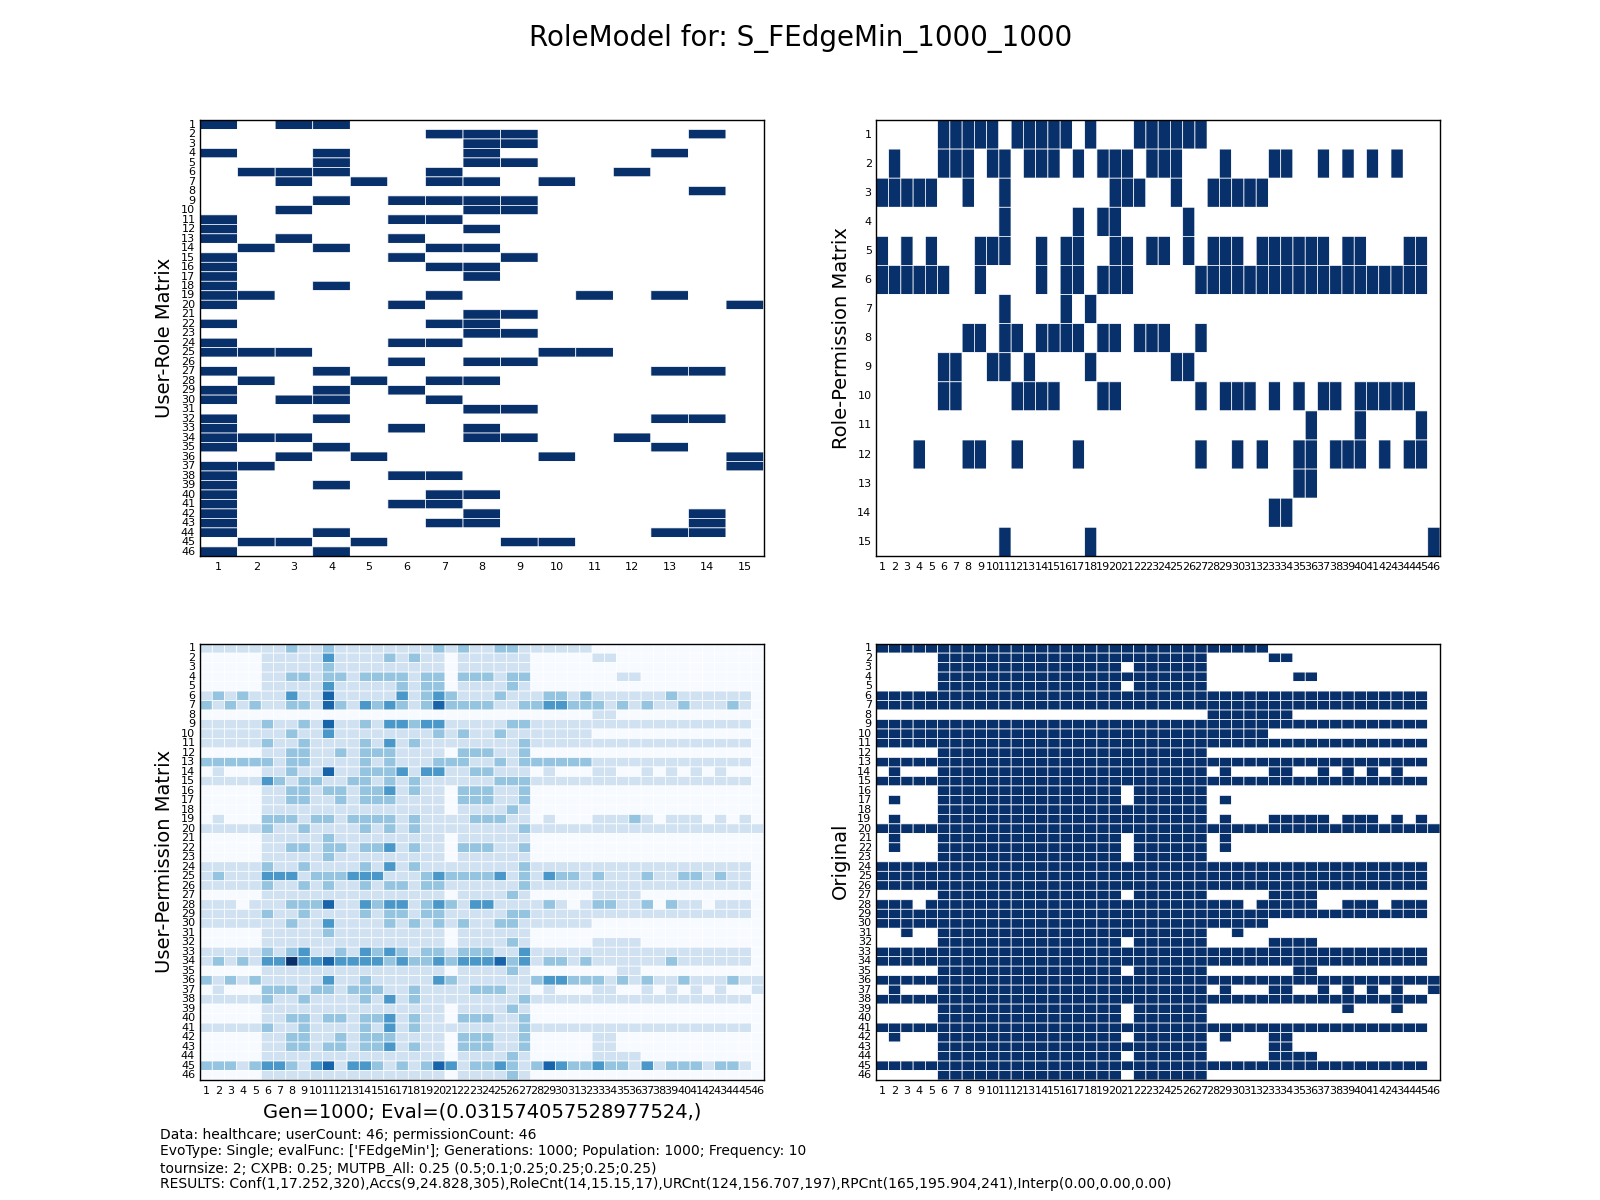
\includegraphics[scale=0.37, trim=4cm 2cm 4cm 2cm, clip=true]{exp5edge_RM}
    \caption{EXPERIMENT 5b: Example of fitness-optimal solution role model resulting of EvoRoleMiner with Fitness function $F_{edge}^{min}$ on healthcare dataset with setup in table \ref{tab:setup3}. From u.l. to l.r.: User-Role Matrix, Role-Permission Matrix, Resulting User-Permission Matrix, Original User-Permission Matrix from Input. A blue box stands for an assignment. The darker the blue the more usre-role- and role-permission assignments causing the user-permission assignment.}
    \label{fig:exp5edge_RM}
\end{figure}

Another critical point is the diversity of the individuals in the populations. When looking on the role count diversity it can be noted, that the individuals of a population quickly get the same role count size. The boxplot in Figure \ref{fig:exp3a_diversity} visualizes the role count diversity of the individuals in a population in different generations in one of the experiments. The boxplots in the other experiment look similar.

\begin{figure}[H]
	\centering
	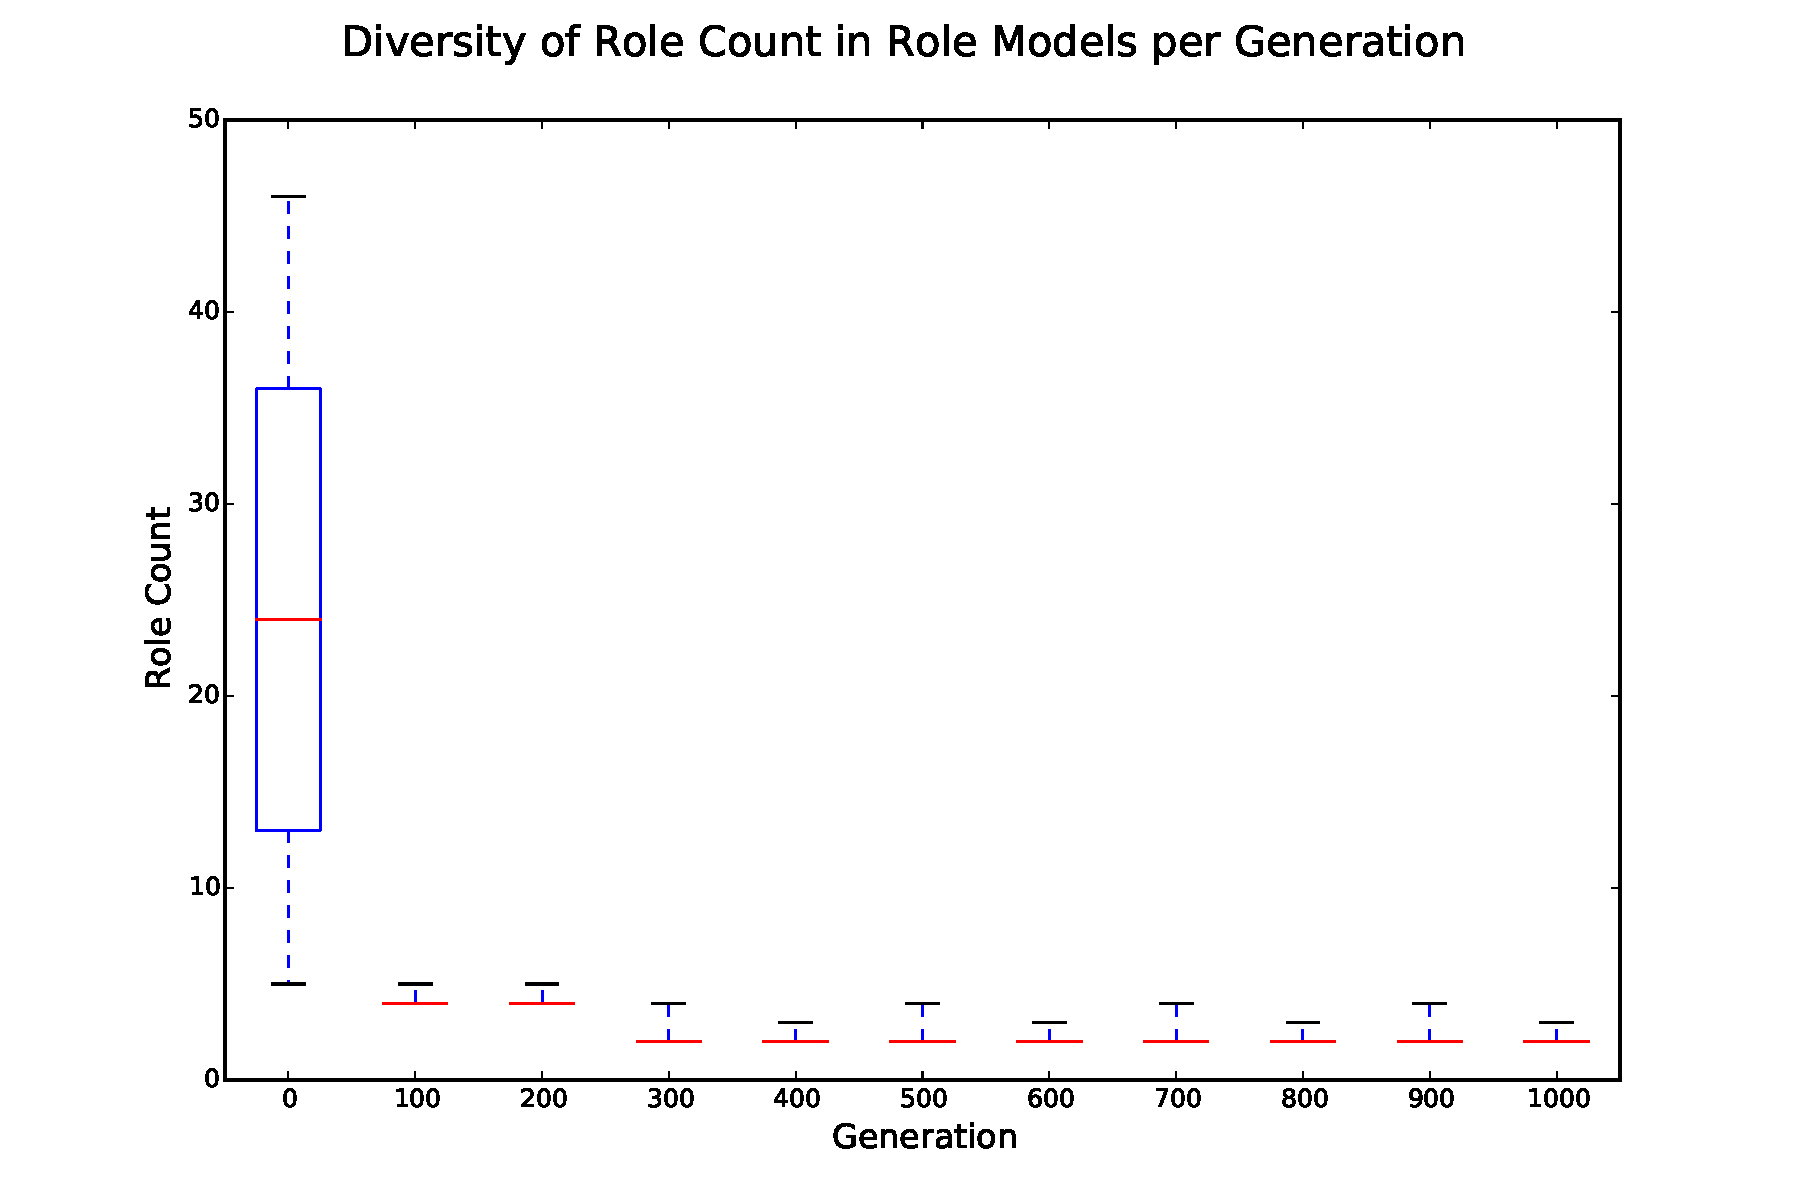
\includegraphics[scale=0.3]{exp3a_diversity}
	\caption{EXPERIMENT 3a: Example boxplot of role count diversity of individuals of a population in different generations.Experiment was executed on the healthcare dataset.}
	\label{fig:exp3a_diversity}
\end{figure}

It is therefore not surprising that it is difficult for the Evo-RoleMiner to find an individual with a minimum amount of violations.